\documentclass[10pt]{beamer}
\usepackage[UTF8]{ctex}
\usepackage{natbib}
\usepackage{commath}%定义d
\usepackage{graphicx}
\graphicspath{{fig/}}
\usepackage{booktabs} % To thicken table lines
\usepackage{bm}
\usepackage{cleveref}
\usepackage{hyperref}

\newcommand\mi{\mathrm{i}}
\newcommand\me{\mathrm{e}}
\usetheme[progressbar=frametitle]{metropolis}

\setsansfont{TimesNewRomanPSMT}
\setmonofont{SFMono-Regular}
\setmainfont{TimesNewRomanPSMT}

\title{第四章\quad 叠加法、热流动和傅立叶分析}
% \subtitle{\small 指导老师:陈十一教授\quad 史一蓬教授}
% \institute{\small 北京大学工学院工程力学专业}
\author{\footnotesize 袁磊祺 \quad 刘志如 \quad 宋庭鉴  \quad 周子铭 \quad 岐亦铭 \quad 董淏翔 \quad  撒普尔}
\date{\today}
%\logo{
\includegraphics[width=5em]{pkured.pdf}}

\setCJKmainfont[ItalicFont=STKaitiSC-Regular,BoldFont=STSongti-SC-Black]{STSongti-SC-Regular}
\setCJKsansfont[ItalicFont=STKaitiSC-Regular,BoldFont=STHeitiSC-Medium]{STHeitiSC-Light}


\begin{document}
  %%%%%%%%%%%%%%%%%%%%%%%%%%%%%%%%%%%%%%%%%%%%%%
\renewcommand\contentsname{\vspace*{-2cm}\centerline{\textsf{目\quad 录}}\vspace*{-1.5cm}}
\renewcommand\listfigurename{插图目录}
\renewcommand\listtablename{表格目录}
\renewcommand\refname{参考文献}
\renewcommand\indexname{索引}
\renewcommand\figurename{图}
\renewcommand\tablename{表}
\renewcommand\abstractname{摘\quad 要}
\renewcommand\partname{部分}
\renewcommand\appendixname{附录}
\def\equationautorefname{式}%
\def\footnoteautorefname{脚注}%
\def\itemautorefname{项}%
\def\figureautorefname{图}%
\def\tableautorefname{表}%
\def\partautorefname{篇}%
\def\appendixautorefname{附录}%
\def\chapterautorefname{章}%
\def\sectionautorefname{节}%
\def\subsectionautorefname{小小节}%
\def\subsubsectionautorefname{subsubsection}%
\def\paragraphautorefname{段落}%
\def\subparagraphautorefname{子段落}%
\def\FancyVerbLineautorefname{行}%
\def\theoremautorefname{定理}%
\crefname{figure}{图}{图}
\crefname{equation}{式}{式}
\crefname{table}{表}{表}



  \maketitle
  \begin{frame}
		\frametitle{目录}
		\tableofcontents{}
\end{frame}

  
\section{热传导方程}

\begin{frame}[allowframebreaks]{叠加原理}

对于线性齐次问题,叠加原理成立。

把齐次问题的解与非齐次问题的一个特解进行线性组合,便可以得到线性非齐次情况的解。

\[Lx=a\]
分解为:
	\[Lx_{i}=0 \] 
	\[Lx_{s}=a\]  
有:
\[x=\sum_{i}x_{i}+x_{s}\]

\end{frame}

\begin{frame}[allowframebreaks]{傅里叶分析严格性}

从数学上看,傅里叶分析级数理论中的关键在于,是否任何函数都能用三角级数表示。

傅里叶分析的早期争议历史,十分典型地表明了纯粹数学和应用数学的侧重点之间的差别。

纯粹数学家手中唯一的武器是清晰而严格的证明,而且只有当所谓定理能够经受的住那个时期所能有的最严厉的批评时,纯粹数学家才会去运用它。

应用数学家决不会对物理证据视而不见。

不顾傅里叶关于热的分析理论的经典著作中缺乏显然的严格性,Kelvin爵士还称它为“一首伟大的数学诗篇”。

傅里叶分析乃是每一位应用数学的学生都应熟悉的一门学科。


\end{frame}

\begin{frame}[allowframebreaks]{定态热传导}

\begin{figure}[htp]
  \centering
  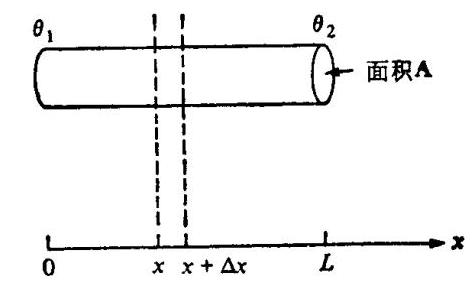
\includegraphics[width=6cm]{1.1.jpeg}
  \caption{沿着一根棒的一维热传导}
  \label{fig:1.1}
\end{figure}


\begin{equation}
\theta=\theta_{s}(x)=\theta_{1}+\left(\theta_{2}-\theta_{1}\right) \frac{x}{L}
\end{equation} 

\begin{equation}
\frac{d \theta_{s}}{d x}=\frac{\theta_{2}-\theta_{1}}{L}
\end{equation}

\begin{equation}
J=-k \frac{d \theta_{s}}{d x}
\end{equation}

其中$k$是导热率系数。

\end{frame}

\begin{frame}[allowframebreaks]{一维热传导的微分方程}


\begin{equation}
J=-k \frac{d \theta}{d x}
\end{equation}

取一小段$x$和$x+\Delta x$之间的一小段圆柱棒研究,穿过$x$处面流入与穿过$x+\Delta x$处面流出,两者相加得到净热量:


\begin{equation}
\dot{q}=A\left [ \left ( k\frac{\partial \theta }{\partial x}\right )_{x+\Delta x}-\left ( k\frac{\partial \theta }{\partial x}\right )_{x}\right ]
\end{equation}

\begin{equation}
\dot{q}=\frac{\partial }{\partial t}\left [ c\theta \rho A\Delta x\right ]
\end{equation}


\begin{equation}
\rho c \frac{\partial \theta}{\partial t}=\frac{\partial}{\partial x}\left(k \frac{\partial \theta}{\partial x}\right)
\end{equation}

均匀材料中,$\kappa =k/\left ( \rho c\right )$
可得:
\begin{equation}
\frac{\partial \theta}{\partial t}=\kappa \frac{\partial^{2} \theta}{\partial x^{2}}
\end{equation}


\end{frame}

\begin{frame}[allowframebreaks]{一维热传导的初始边值问题}

\begin{figure}[htp]
  \centering
  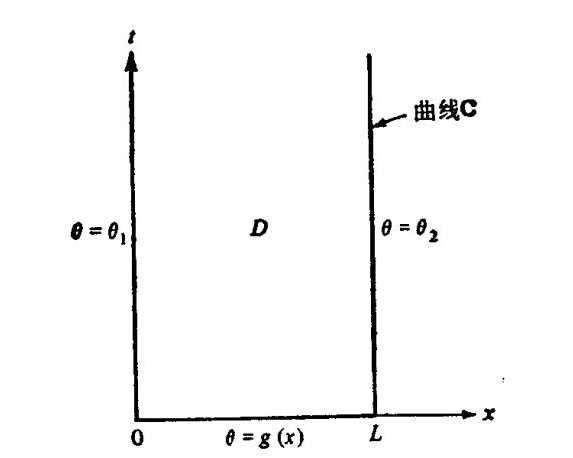
\includegraphics[width=6cm]{1.2.jpeg}
  \caption{热传导问题的数学表述:域,它的边界,边界条件}
  \label{fig:1.2}
\end{figure}

\begin{equation}
\frac{\partial \theta}{\partial t}=\kappa \frac{\partial^{2} \theta}{\partial x^{2}}, 0<x<L, 0<t<\infty
\end{equation}

\begin{equation}
\theta(x, 0)=g(x), 0<x<L
\end{equation}

\begin{equation}
\theta(0, t)=\theta_{1}, \theta(L, t)=\theta_{2}, t>0
\end{equation}

\begin{columns}
  \column{0.5\textwidth}

  \begin{figure}[htp]
    \centering
    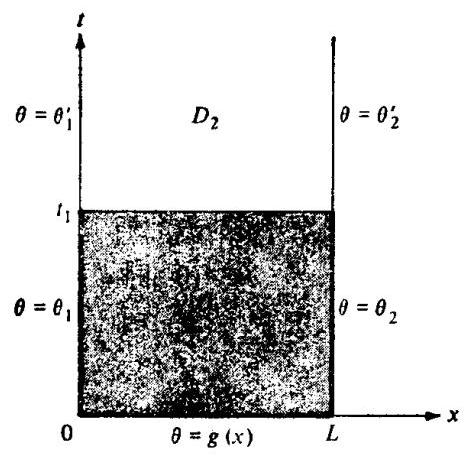
\includegraphics[width=5cm]{1.3.jpeg}
    \caption{由边界条件的变化所示明的过去和
    将来之间的区別. 对于 $t<t_{1},$ 解只受到粗
    线勾划出的边界 $C_{1}$ 上的变化的影响.}
    \label{fig:1.3}
  \end{figure}
  

  \column{0.5\textwidth}
  \begin{figure}[htp]
    \centering
    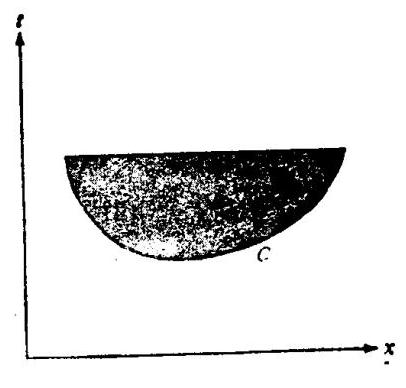
\includegraphics[width=5cm]{1.4.jpeg}
    \caption{热传导问题的一般数学表述:域和它的边界.}
    \label{fig:1.4}
  \end{figure}
\end{columns}


\end{frame}

\begin{frame}[allowframebreaks]{三维热传导方程}

\begin{equation}
\rho c \frac{\partial \theta}{\partial t}=\mathbf{\nabla} \cdot(k \nabla \theta)
\end{equation}

\begin{equation}
\frac{\partial}{\partial t} \iiint_{R} c \rho \theta d \tau=\iint_{\partial R} k \frac{\partial \theta}{\partial n} d \sigma=\iint_{\partial_{R}} k \mathbf{n} \cdot \nabla \theta d \sigma
\end{equation}

	
\begin{equation}
\iiint_{R}\left[c \rho \frac{\partial \theta}{\partial t}-\nabla \cdot(k \nabla \theta)\right] d \tau=0
\end{equation}

\end{frame}

\begin{frame}[allowframebreaks]{三类边界条件}

\begin{enumerate}
  \item 规定了边界上所有时刻的对应温度即,在某一边界上$\theta  =a\left ( t\right )$
  \item 边界是绝热的,边界上有$\frac{\partial \theta }{\partial n}=0$
  \item 从边界上散失掉的热量正比于表面温度高于环境温度的温差$\frac{\partial \theta }{\partial n}=h\left ( \theta -\theta _{0}\right )$
\end{enumerate}

\end{frame}

\begin{frame}[allowframebreaks]{唯一性定理}

假设$\theta _{1}\left ( x,y,z,t\right )$与$\theta _{2}\left ( x,y,z,t\right )$都是方程的解,我们取$\theta =\theta _{2}-\theta _{1}$

由$\rho c \frac{\partial \theta}{\partial t}=\mathbf{\nabla} \cdot(k \nabla \theta)$可得

\begin{equation}
\frac{1}{2}\rho c\frac{\partial \theta ^{2}}{\partial t}=k\theta \Delta \theta  =k\left ( \nabla \cdot \left (\theta  \nabla \theta  \right )-\left ( \nabla\theta \right )^{2}\right )
\end{equation}

\begin{equation}\frac{1}{2}\iiint _{R}\rho c\frac{\partial \theta ^{2}}{\partial t}d\tau =\iint_{\partial R}k\theta \frac{\partial \theta }{\partial n}d\sigma -\iiint _{R}k\left ( \nabla\theta \right )^{2}d\tau 
\end{equation}

\end{frame}

\begin{frame}[allowframebreaks]{极大值原理}


\begin{alertblock}{物理直觉}
  \vspace{3pt}
  热量的扩散是从高温到低温处移动,应该不会由于扩散使得热量的堆积,所以我们认为在一内部区域内的温度不会超过出现在边界上的最高温度或者初始时刻给定的最高温度。
\end{alertblock}

\begin{alertblock}{数学证明}
  \vspace{3pt}
  首先,事实上物理意义与直观无法提供证明思路。
  
  证明过程分为两步:
  \begin{enumerate}
    \item 证明热传导方程的平均值性质,
    \item 用平均值性质证明有界区域最大值原理。
  \end{enumerate}
\end{alertblock}

\end{frame}

\section{分离变量法}

\begin{frame}[allowframebreaks]{控制方程}

为满足叠加原理,从而使用傅里叶方法,需将定态解从解中分离,建立瞬态解的方程:
\begin{equation}
v(x, t)=\theta(x, t)-\theta_{s}(x)
\end{equation}	
\begin{equation}
\frac{\partial v}{\partial t}=\kappa \frac{\partial^{2} v}{\partial x^{2}}
\end{equation}
初始条件:
\begin{equation}
0<x<L, v(x, 0)=f(x) ; f(x)=g(x)-\theta_{s}(x)
\end{equation}
边界条件:
\begin{equation}
v(0, t)=v(L, t)=0, \text { 对于所有 } t>0
\end{equation}


\end{frame}

\begin{frame}[allowframebreaks]{乘积解}

把解写为乘积解形式:
\begin{equation}
v(x, t)=X(x) T(t)
\end{equation}
代入原微分方程:
\begin{equation}
\frac{X^{\prime \prime}(x)}{X(x)}=\frac{T^{\prime}(t)}{\kappa T(t)}
\end{equation}
\begin{equation}
X^{\prime \prime}=k X, T^{\prime}=k \kappa T
\end{equation}


经讨论:\begin{equation}k=-\alpha^2\end{equation}
\begin{equation}
X=C_{1} \cos \alpha x+C_{2} \sin \alpha x
\end{equation}
乘积解边界条件:
\begin{equation}
X(0) T(t)=0, X(L) T(t)=0 \text { 对所有 } t>0
\end{equation} 

\begin{equation}
X(0)=X(L)=0
\end{equation}
\begin{equation}
C_{1}=0
\end{equation}
\begin{equation}
C_{2} \sin \alpha L=0
\end{equation}

\begin{equation}
\alpha=m \pi / L, m=1,2,3, \cdots
\end{equation}
\begin{equation}
X(x)=B_{m} \sin \frac{m \pi x}{L}, B_{m} \text { 为任意常数 }
\end{equation}

代入方程:\begin{equation}T^{\prime}=k \kappa \end{equation}
\begin{equation}
T^{\prime}=-\frac{m^{2} \pi^{2}}{L^{2}} \kappa T
\end{equation}

因此可得到:
\begin{equation}
v(x, t)=\sum_{m=1}^{\infty} B_{m} \sin \frac{m \pi x}{L} \exp \left(-\frac{m^{2} \pi^{2}}{L^{2}} \kappa t\right)
\end{equation}


\end{frame}

\begin{frame}[allowframebreaks]{乘积解的系数}

运用初始条件:
\begin{equation}
f(x)=\sum_{m=1}^{\infty} B_{m} \sin \frac{m \pi x}{L}, 0<x<L
\end{equation}
定义内积:
\begin{equation}
(f, g)=\int_{0}^{L} f(x) g(x) d x
\end{equation}
由三角函数的正交性,可得到:
\begin{equation}
B_{m}=2 L^{-1}\left(f(x), \sin \frac{m \pi x}{L}\right)
\end{equation}
最终得到方程的解为:
\begin{equation}
\theta(x, t)=\theta_{s}(x)+\sum_{m=1}^{\infty} B_{m}\left(\sin \frac{m \pi x}{L}\right) e^{-(m \pi / L)^{2} \kappa t}
\end{equation}

\end{frame}

\begin{frame}[allowframebreaks]{观察与发现}

将方程和解无量纲化:
\begin{equation}
\xi=x L^{-1},\tau=\kappa t L^{-2}
\end{equation}
\begin{equation}
\Theta(\xi, \tau)=\theta\left(L \xi, t_{0} \tau\right)=\theta_{s}(L \xi)+\sum_{m=1}^{\infty} B_{m} \sin m \pi \xi \cdot e^{-(m \pi)^{2} \tau}
\end{equation}
\begin{equation}
\frac{\partial \Theta}{\partial \tau}=\frac{\partial^{2} \Theta}{\partial \xi^{2}}
\end{equation}
求解域为:	
\begin{equation}
D^{\prime}: 0<\xi<1,0<\tau<\infty
\end{equation}
初始和边界条件分别为:
\begin{equation}
\begin{array}{c}
\Theta(0, t)=\Theta(1, t)=0 \\
\Theta(\xi, 0)=G(\xi), \text { 其中 } G(\xi)=g(L \xi)
\end{array}
\end{equation}
该方程不显式依赖于材料属性
相似性:对同种材料,长度变为$N$倍,时间变为$N^2$倍。

$m=1$的解衰减速度最慢,衰减因子为$ e^{-\pi^{2}\kappa t/4d^{2}}$,在$t=d^{2}/\kappa$时间内,峰值衰减到$0.08$,可以认为,这时间$t$内,“一种物质”大约扩散了$(\kappa t)^{1/2}$个距离单位。

\end{frame}

\section{傅立叶定理}

\begin{frame}{傅立叶定理}
  在区间$(0,L)$中任何合理的函数$f(x)$都可以用一个傅立叶正弦级数来表示,并且级数在两个端点的值为0
  \begin{equation}
    f(x)=\frac{x}{L}\left(1-\frac{x}{L}\right)
  \end{equation}
  \begin{equation}
    f(x) = 1
  \end{equation}
\end{frame}

\begin{frame}[allowframebreaks]{傅立叶正弦级数的加法}
  \begin{equation}
    S_{N}(x)=\frac{2}{\pi} \int_{0}^{\pi} K_{N}(x, \xi) f(\xi) \dif  \xi,\quad 0<x<\pi
    \label{eq:2Sn}
  \end{equation}
  其中
  \begin{equation}
    K_{N}(x, \xi)=\sum_{m=1}^{N} \sin (m x) \sin (m \xi),\quad 0<x, \xi<\pi
  \end{equation}
  利用
  \begin{equation}
    \sin w=\frac{\me^{\mi w}-\me^{-\mi w}}{2 \mi}
  \end{equation}
  可得
  \begin{equation}
    K_{N}(x, \xi)=\frac{1}{2}\left\{\frac{\sin \left[\left(N+\frac{1}{2}\right)(x-\xi)\right]}{2 \sin \left[\frac{1}{2}(x-\xi)\right]}-\frac{\sin \left[\left(N+\frac{1}{2}\right)(x+\xi)\right]}{2 \sin \left[\frac{1}{2}(x+\xi)\right]}\right\}
    \label{eq:2Kn}
  \end{equation}

  \begin{figure}
    \centering
    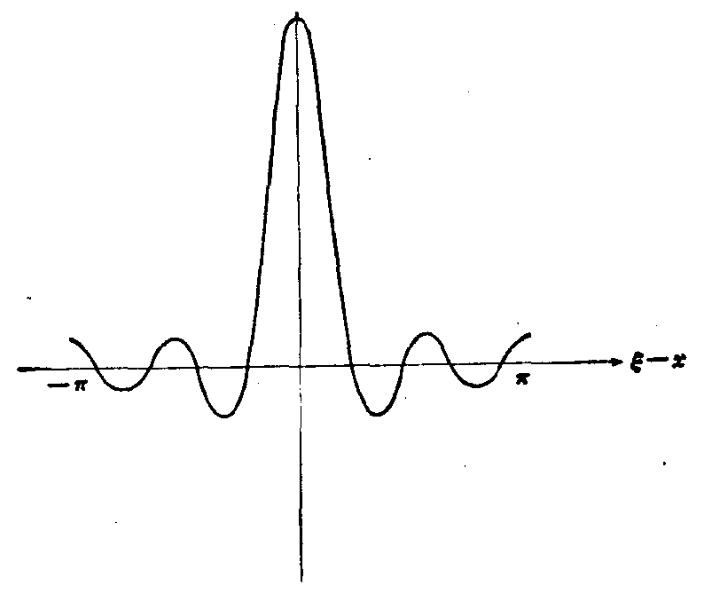
\includegraphics[width=7cm]{21.png}
    \caption{函数$\frac{\sin \left[\left(N+\frac{1}{2}\right)(x-\xi)\right]}{2 \sin \left[\frac{1}{2}(x-\xi)\right]}$的示意图}
    \label{fig:21}
  \end{figure}
  
  把\cref{eq:2Kn}代入\cref{eq:2Sn}可得
  \begin{equation}
    S_{N}(x)=S_{N}^{(1)}(x)+S_{N}^{(2)}(x),\quad 0<x<\pi
  \end{equation}
  其中
  \begin{gather}
    S_{N}^{(1)}(x)=\frac{1}{\pi} \int_{0}^{\pi} \frac{\sin \left[\left(N+\frac{1}{2}\right)(x-\xi)\right]}{2 \sin \left[\frac{1}{2}(x-\xi)\right]} f(\xi) \dif \xi \\
    S_{N}^{(2)}(x)=-\frac{1}{\pi} \int_{0}^{\pi} \frac{\sin \left[\left(N+\frac{1}{2}\right)(x+\xi)\right]}{2 \sin \left[\frac{1}{2}(x+\xi)\right]} f(\xi) \dif \xi
  \end{gather}



  \metroset{block=fill}

  \begin{block}{引理1}
      若  $\phi(x)$   在闭区间 $[a,  b]$ 内分段光滑,则
    \begin{equation}
      \int_{a}^{b} \phi(\xi) \underset{}{ } \begin{array}{c}
        \sin  \\
        \cos \\
    \end{array}\lambda \xi \dif \xi=O\left(\lambda^{-1}\right),\ \text {当 }\ \lambda \rightarrow \infty
    \end{equation}
  \end{block}

  \begin{block}{引理2}
      若  $\phi(x)$   在闭区间 $[a,  b]$ 内分段光滑,在$x_0$连续,则
      \begin{equation}
        \lim _{\lambda \rightarrow \infty} \int_{a}^{b} \phi(\xi) \frac{\sin \left[\lambda\left(x_{0}-\xi\right)\right]}{x_{0}-\xi} \dif \xi=\pi \phi\left(x_{0}\right),\ \text { 当 }\ a<x<b .
        \label{eq:2-lemma2}
      \end{equation}
  \end{block}

  \begin{block}{引理3}
    若在点 $x_{0}$ 处 $, \phi(x)$ 有一个跳跃间断,\cref{eq:2-lemma2}仍然适用,只要我们把 $\phi\left(x_{0}\right)$ 定义为 $\phi(\xi)$ 在 $\xi \rightarrow x_{0}$ 时的左、右极限的 平均:
    \begin{equation}
      \phi\left(x_{0}\right)=\frac{1}{2}\left[\phi\left(x_{0}-0\right)+\phi\left(x_{0}+0\right)\right]
    \end{equation}
    这里,有定义
    \begin{equation}
      \phi\left(x_{0} \pm 0\right)=\lim _{\varepsilon \downarrow 0} \phi\left(x_{0} \pm \varepsilon\right)
    \end{equation}
    指向下的箭头意味着 $\varepsilon$ 递减至零; 即, $\varepsilon$ 通过正值趋近于0
\end{block}

由引理1得$S_{N}^{(2)}(x)\to 0$. 根据引理2,如果定义
\begin{equation}
  \phi(\xi)=f(\xi) \frac{x-\xi}{2 \sin \left[\frac{1}{2}(x-\xi)\right]}
\end{equation}
则有$S_{N}^{(1)}(x)\to f(x)$, 如果在$x=x_0,\ f(x)$不连续,则在$x_0$处的正弦级数的和是
\begin{equation}
  f\left(x_{0}\right)=\frac{1}{2}\left[f\left(x_{0}+0\right)+f\left(x_{0}-0\right)\right].
\end{equation}

\end{frame}

\begin{frame}[allowframebreaks]{全空间的傅立叶级数}
  由傅立叶级数定义的函数是周期的
  \begin{equation}
    f(x+2 \pi)=f(x)
  \end{equation}
  全空间的傅立叶级数
  \begin{equation}
    f(x) \sim \frac{1}{2} a_{0}+\sum_{n=1}^{\infty}\left(a_{n} \cos n x+b_{n} \sin n x\right),\quad -\pi<x<\pi
    \label{eq:2fuli}
  \end{equation}
  其中
  \begin{equation}
    a_{n}=\frac{1}{\pi} \int_{-\pi}^{\pi} f(x) \cos n x \dif x, \quad b_{n}=\frac{1}{\pi} \int_{-\pi}^{\pi} f(x) \sin n x \dif x
    \label{eq:2fuli2}
  \end{equation}
  级数\cref{eq:2fuli}也常常取复数形式
\begin{equation}
  f(x) \sim \sum_{-\infty}^{\infty} c_{n} \me^{i n x}
\end{equation}
其中
\begin{equation}
  c_{n}=\frac{1}{2 \pi} \int_{-\pi}^{\pi} f(x) \me^{-\mi n \xi} \dif \xi
\end{equation}
其中
\begin{equation}
  c_{0}=a_{0} / 2, \quad c_{n}=\frac{1}{2}\left(a_{n}-\mi b_{n}\right)
\end{equation}
\end{frame}

\begin{frame}{傅立叶级数的加法}
  \metroset{block=fill}

  \begin{block}{定理}
  如果 $f(x)$ 在区间$(-\pi, \pi)$ 内分段光滑,那么它的傅 里叶级数——如在\cref{eq:2fuli}和\cref{eq:2fuli2}所定义的,在 $x=x_{0}$ 处收敛于
  \begin{equation}
    f\left(x_{0}\right)=\frac{1}{2}\left[f\left(x_{0}-0\right)+f\left(x_{0}+0\right)\right]
  \end{equation}
在端点,这一级数收敛于 $\frac{1}{2}[f(-\pi+0)+f(\pi-0)]$。
  \end{block}
\end{frame}


\section{傅立叶级数的性质}


\begin{frame}[allowframebreaks]
  \frametitle{傅里叶级数简单示例}
  
  方形波函数
  \begin{equation}
  S(x)=\frac{4}{\pi}\left(\sin x+\frac{1}{3} \sin 3 x+\frac{1}{5} \sin 5 x+\cdots\right)
  \end{equation}
  
  绝对值函数
  \begin{equation}
  C(x)=|x|=\pi-\frac{4}{\pi}\left(\frac{\cos x}{1^{2}}+\frac{\cos 3 x}{3^{2}}+\frac{\cos 5 x}{5^{2}}+\cdots\right)
  \end{equation}
  
  \begin{equation}
  C^{\prime}(x)=S(x)
  \end{equation}
  \end{frame}
  
  \begin{frame}[allowframebreaks]
  \frametitle{傅里叶级数的积分和微分}
  
  分段光滑的函数可用下面的傅里叶级数表示
  \begin{equation}
  f(x)=\frac{a_{0}}{2}+\sum_{n=1}^{\infty}\left(a_{n} \cos n x+b_{n} \sin n x\right)
  \end{equation}
  
  形式积分
  \begin{equation}
  \int_{0}^{x} f(t) d t-\frac{a_{0}}{2} x \sim \sum_{n=1}^{\infty}\left[\frac{a_{n}}{n} \sin n x+\frac{b_{n}}{n}(1-\cos n x)\right]
  \end{equation}
  
  可用下式验证
  \begin{equation}
  \int_{0}^{x} f(t) d t-\frac{a_{0}}{2} x=\frac{A_{0}}{2}+\sum_{n=1}^{\infty}\left(A_{n} \cos n x+B_{n} \sin n x\right)
  \end{equation}
  
  形式微分
  \begin{equation}
  f^{\prime}(x) \sim 0+\sum_{n=1}^{\infty}\left(-n a_{n} \sin n x+n b_{n} \cos n x\right)
  \end{equation}
  
  若用下式验证
  \begin{equation}
  \frac{a_{0}^{\prime}}{2}+\sum_{n=1}^{\infty}\left(a_{n}^{\prime} \cos n x+b_{n}^{\prime} \sin n x\right)
  \end{equation}
  
  得约束条件之一
  \begin{equation}
  f(\pi)=f(-\pi)
  \end{equation}
  \end{frame}
  
  \begin{frame}[allowframebreaks]
  \frametitle{吉布斯现象}
  
  部分和在间断点附近出现称作吉布斯现象的异常行为
  
  以方波函数为例,可证明,仅当N趋于无穷时,部分和才会趋近于极限值
  
  \begin{equation}
  S_{N}(x) \approx \frac{2}{\pi} \int_{0}^{m x} \frac{\sin \eta}{\eta} \frac{\eta / 2 m}{\sin (\eta / 2 m)} d \eta
  \end{equation}
  
  其中
  \begin{equation}
  m=N+\frac{1}{2}
  \end{equation}
  
  \begin{equation}
  S_{\max }=\frac{2}{\pi}\left(\int_{0}^{\left(N+\frac{1}{2}\right) x} \frac{\sin \eta}{\eta} d \eta\right)_{\max } \approx 1.179
  \end{equation}
  
  \begin{figure}[htp]
    \centering
    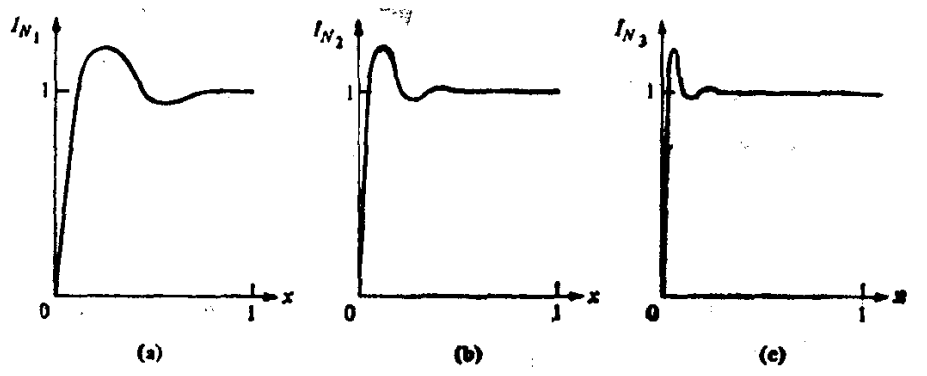
\includegraphics[width=10cm]{31.png}
    \caption{$I_N(x)$的定性图像}
    \label{fig:3.1}
  \end{figure}
  
\end{frame}
  
  \begin{frame}[allowframebreaks]
  \frametitle{具有最小二乘误差的近似}
  
  均方误差取极小值
  \begin{equation}
  M=\frac{1}{2 \pi} \int_{-\pi}^{\pi} \varepsilon_{N}^{2} d x
  \end{equation}
  
  \begin{equation}
  \varepsilon_{N}=f(x)-\sum_{n=-N}^{N} \gamma_{n} e^{i n x}
  \end{equation}
  
  必要条件
  \begin{equation}
  \gamma_{n}=\frac{1}{2 \pi} \int_{-\pi}^{\pi} f(x) e^{-i n x} d x
  \end{equation}
  
  充分条件
  \begin{equation}
  c_{n}=\gamma_{n}
  \end{equation}
  \end{frame}
  
  \begin{frame}[allowframebreaks]
  \frametitle{具有最小二乘误差的近似}
  
  最小二乘法可推广
  
  正交条件
  \begin{equation}
  \int_{-\pi}^{\pi} \phi_{m}(x) \phi_{n}(x) w(x) d x=\delta_{m n}
  \end{equation}
  
  其中$w$为非负的权函数
  
  加权均方误差取最小值
  \begin{equation}
  \varepsilon_{N}=f(x)-\sum_{n=0}^{N} \gamma_{n} \phi_{n}(x)
  \end{equation}
  
  \begin{equation}
  M_{w}=\frac{\int_{-\pi}^{\pi} \varepsilon_{N}^{2}(x) w(x) d x}{\int_{-\pi}^{\pi} w(x) d x}
  \end{equation}
  \end{frame}
  
  \begin{frame}[allowframebreaks]
  \frametitle{贝塞尔不等式和Parseval定理}
  
  \begin{equation}
  M=\left\langle f\ ^{2}\right\rangle-\sum_{n=-N}^{N}\left|c_{n}\right|^{2}+\sum_{n=-N}^{N}\left|c_{n}-\gamma_{n}\right|^{2}
  \end{equation}
  
  由于条件$c_{n}=\gamma_{n}$和$M \geq 0$
  
  \begin{equation}
  \sum_{n=-N}^{N}\left|c_{n}\right|^{2} \leq\left\langle f\ ^{2}\right\rangle
  \end{equation}
  
  假如除了有限多个间断点意外,傅里叶级数按点态方式收敛,则
  \begin{equation}
  \lim _{N \rightarrow \infty} M=0
  \end{equation}
  
  \begin{equation}
  \sum_{n=-\infty}^{\infty}\left|c_{n}\right|^{2}=\left\langle f\ ^{2}\right\rangle
  \end{equation}
  
  Riesz-Fischer定理是Parseval定理的逆问题
  \begin{equation}
  \frac{1}{2} a_{0}^{2}+\sum_{m=1}^{\infty}\left(a_{m}^{2}+b_{m}^{2}\right)
  \end{equation}
  
  \begin{equation}
  \frac{a_{0}}{2}+\sum_{m=1}^{\infty}\left(a_{m} \cos m x+b_{m} \sin m x\right)
  \end{equation}
  
  \end{frame}
  
  \begin{frame}[allowframebreaks]
  \frametitle{Parseval定理的应用举例}
  
  根据普朗克辐射定律计算斯蒂芬辐射常数时,需要计算积分
  \begin{equation}
  I=\int_{0}^{\infty} \frac{x^{3}}{e^{x}-1} d x
  \end{equation}
  
  \begin{equation}
  1+\frac{1}{3^{4}}+\frac{1}{5^{4}}+\cdots=\frac{\pi^{4}}{96}
  \end{equation}
  
  \begin{equation}
  I=\Gamma(4)\left(1+\frac{1}{2^{4}}+\frac{1}{3^{4}}+\cdots\right)
  \end{equation}
  
  \begin{equation}
  I=\frac{\frac{\pi^{4}}{96}}{1-\frac{1}{2^{4}}} \times 6=\frac{\pi^{4}}{15}
  \end{equation}
  \end{frame}

\end{document}